%!TEX TS-program = xelatex  
%!TEX encoding = UTF-8 Unicode  

\documentclass[12pt]{article}  
\usepackage{geometry}  
\geometry{letterpaper}  
\usepackage{fancyhdr}
\usepackage{extramarks}
\usepackage{amsmath}
\usepackage{amsthm}
\usepackage{amsfonts}
\usepackage{tikz}
\usepackage[plain]{algorithm}
\usepackage{algpseudocode} 
\usepackage{caption}
\usepackage{booktabs}
\usepackage{graphics}
\usepackage{amsmath}
\usepackage{amsfonts}

\usepackage{xltxtra,fontspec,xunicode}
\usepackage[slantfont,boldfont]{xeCJK}
%\setCJKmainfont{宋体}   
\setmainfont{Optima}   
\defaultfontfeatures{Mapping=tex-text}  

\usepackage{xltxtra,fontspec,xunicode}
\usepackage[slantfont,boldfont]{xeCJK}
%\setCJKmainfont{宋体}   
\setmainfont{Optima}   
\defaultfontfeatures{Mapping=tex-text}  

\XeTeXlinebreaklocale “zh”  
\XeTeXlinebreakskip = 0pt plus 1pt minus 0.1pt   
 
\usepackage{listings}
\usepackage{color}
\definecolor{dkgreen}{rgb}{0,0.6,0}
\definecolor{gray}{rgb}{0.5,0.5,0.5}
\definecolor{mauve}{rgb}{0.58,0,0.82}

\lstset{frame=tb,
  language=Java,
  aboveskip=3mm,
  belowskip=3mm,
  showstringspaces=false,
  columns=flexible,
  basicstyle={\small\ttfamily},
  numbers=none,
  numberstyle=\tiny\color{gray},
  keywordstyle=\color{blue},
  commentstyle=\color{dkgreen},
  stringstyle=\color{mauve},
  breaklines=true,
  breakatwhitespace=true,
  tabsize=3
} 

\topmargin=-0.45in
\evensidemargin=0in
\oddsidemargin=0in
\textwidth=6.5in
\textheight=9.0in
\headsep=0.25in

\linespread{1.1}

\pagestyle{fancy}
\lhead{\hmwkAuthorName}
\rhead{\hmwkClass}
\chead{\hmwkTitle}

\renewcommand\headrulewidth{0.4pt}
\renewcommand\footrulewidth{0.4pt}

\setlength\parindent{0pt}

% Homework Details

\newcommand{\hmwkTitle}{homework\ \#5}
\newcommand{\hmwkClass}{Deep Reinforcement Learning}
\newcommand{\hmwkAuthorName}{Tianxiao Hu}


\begin{document}
\pagebreak

\section{Problem 1}
\begin{figure}[!h]
\centering
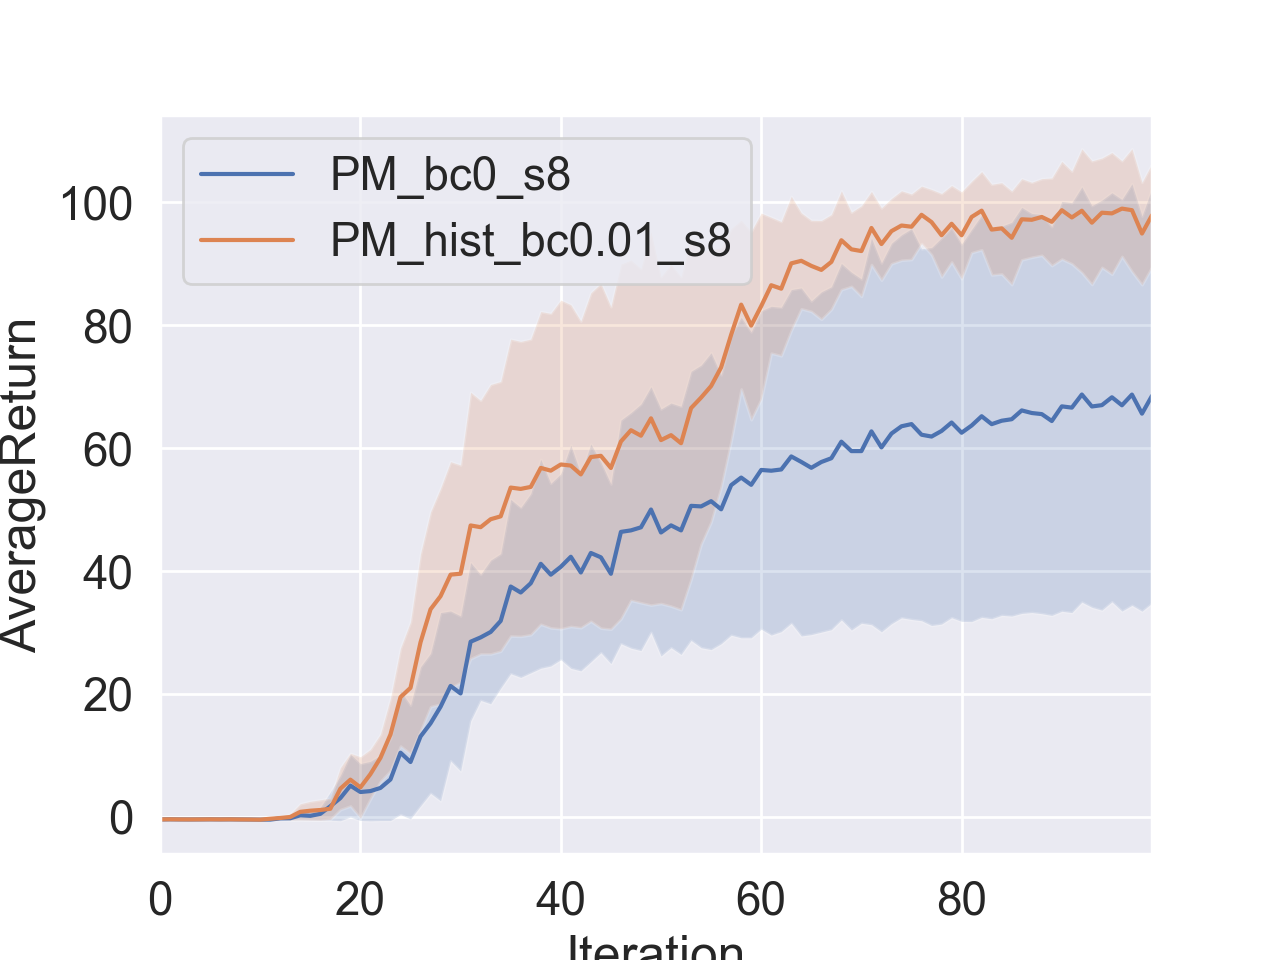
\includegraphics[width=5in]{1.png}
\caption{Comparison for agent with histogram-based exploration
and agent with no exploration for PointMass.}
\end{figure}

\newpage

\section{Problem 2}
\begin{figure}[!h]
\centering
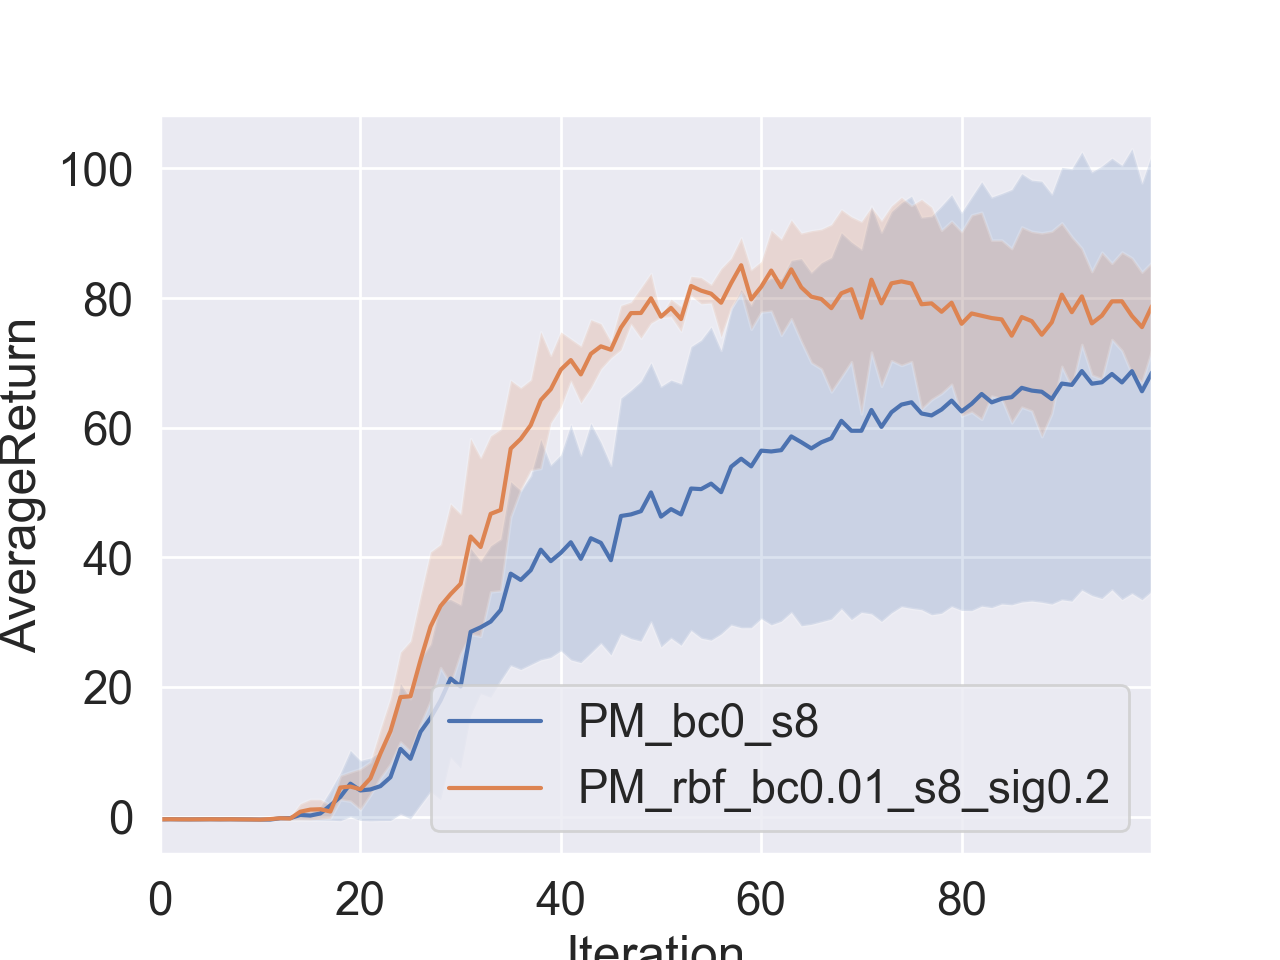
\includegraphics[width=5in]{2.png}
\caption{Comparison for agent with KDE-based exploration and agent with no exploration for PointMass.}
\end{figure}

\newpage

\section{Problem 3}
\begin{figure}[!h]
\centering
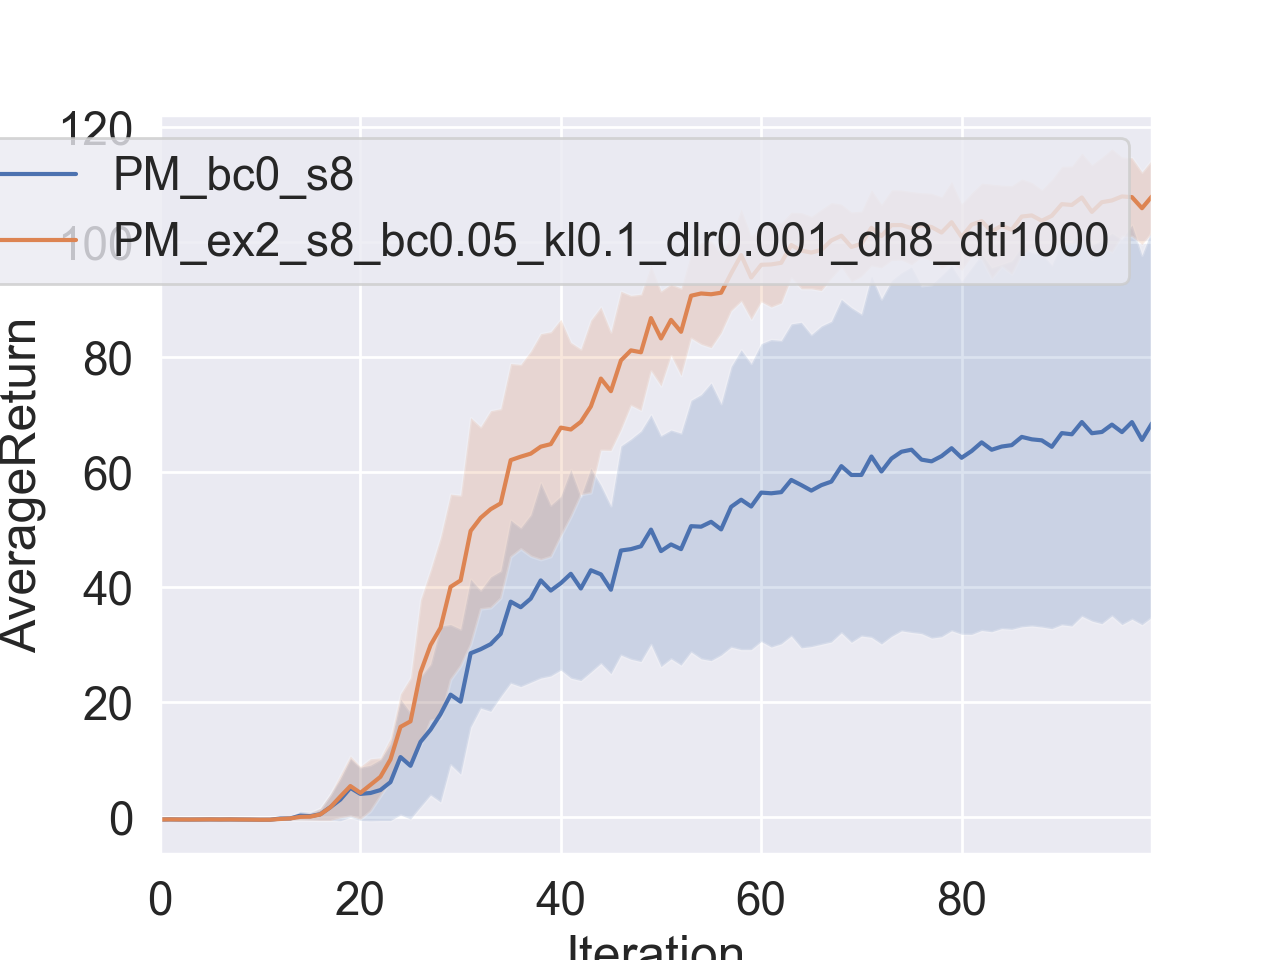
\includegraphics[width=5in]{3.png}
\caption{Comparison for agent with EX2-based exploration and
agent with no exploration for PointMass.}
\end{figure}

\newpage

\section{Problem 4}
\begin{figure}[!h]
\centering
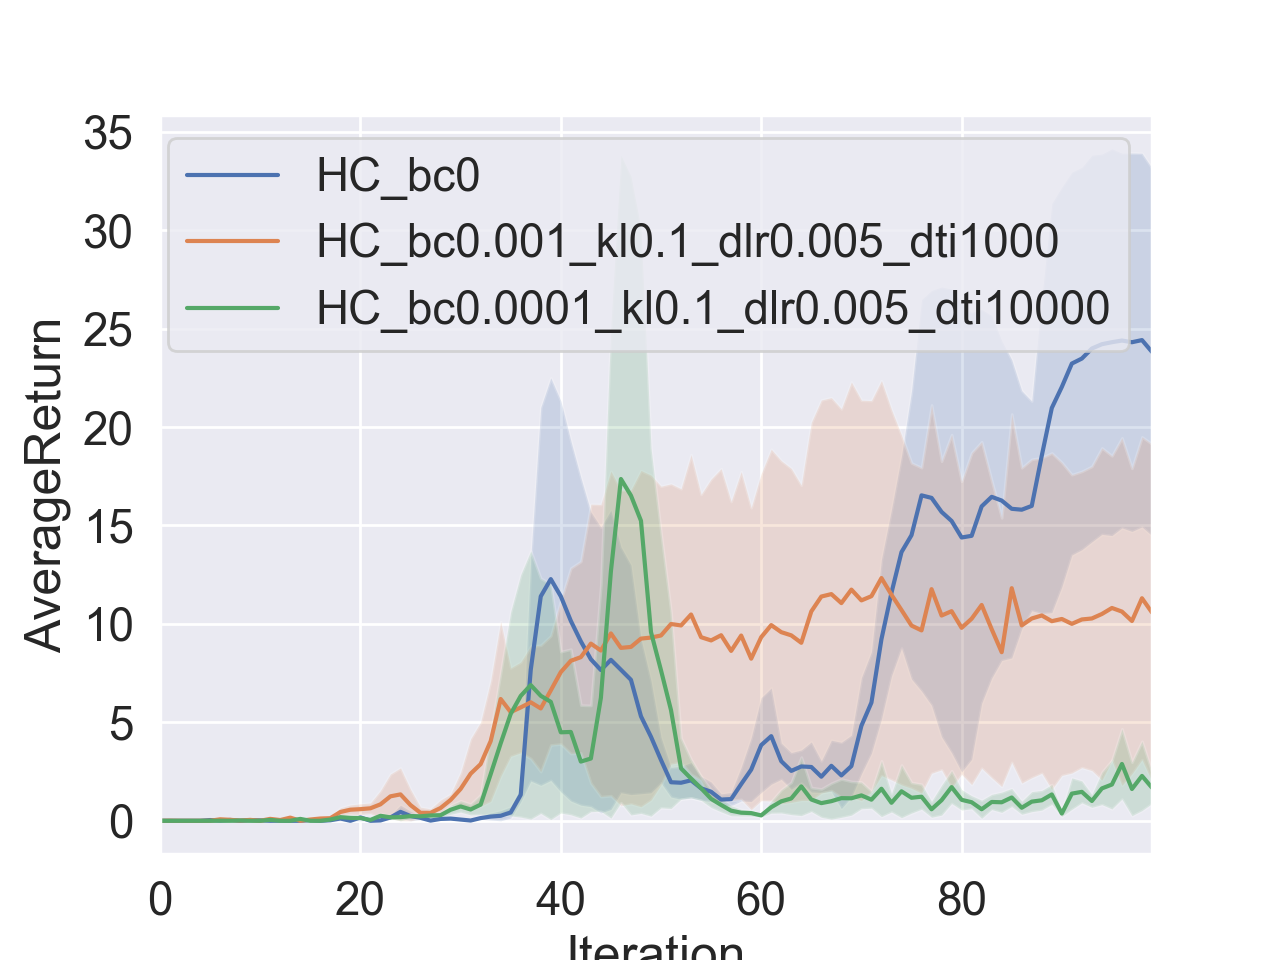
\includegraphics[width=5in]{4.png}
\caption{Comparison for two agents with EX2-based exploration and
another agent with no exploration for HalfCheetah.}
\end{figure}
(1)The learning curve is going up and down is because that even after the agents have already reached the optimal states, they are still incentivized by the reward bonus to explore somewhere else. Thus the agents wouldn't stop exploring, which would result in suboptimal returns.

(2)Different bonus parameter will affect agent's performance. A bigger bonus parameter will keep driving the agent to explore somewhere else and have a different learning curve.
\newpage
\end{document}  
  